\documentclass{beamer}
\colorlet{structure}{green!50!black}

\mode<article> % only for the article version
{
  \usepackage{fullpage}
  \usepackage{hyperref}
}
\mode<presentation>
{
	\setbeamertemplate{background canvas}[vertical shading][bottom=red!10,top=blue!10]
%	\useinnertheme[shadow=true]{rounded}
%	\useoutertheme{shadow}
%	\usecolortheme{whale}
	\setbeamerfont{block title}{size={}}
  \usefonttheme[onlysmall]{structurebold}
}

\setbeamersize{mini frame size=5cm}

\usepackage[english]{varioref}

\usetheme{Hannover}
\usecolortheme{dove}
%\setbeamercolor{math text}{fg=green!50!black}
%\setbeamercolor{normal text in math text}{parent=math text}

%\usepackage{pgf,pgfarrows,pgfnodes,pgfautomata,pgfheaps,pgfshade}
\usepackage{amsmath,amssymb}
%\usepackage[latin1]{inputenc}
\usepackage[utf8]{inputenc}
\usepackage{colortbl}
\usepackage[english,german,ngerman]{babel}
% Line spacing
\usepackage{setspace}
\usepackage{listings}
%\usepackage{lmodern}
%\usepackage[T1]{fontenc}
\usepackage{times}
\setbeamercovered{dynamic}

%
% The following defintions are peculiar to this particular
% presetation. They have nothing to do with the beamer class
%

\newcommand{\Lang}[1]{\operatorname{\text{\textsc{#1}}}}

\newcommand{\Class}[1]{\operatorname{\mathchoice
  {\text{\normalfont\small #1}}
  {\text{\normalfont\small #1}}
  {\text{\normalfont#1}}
  {\text{\normalfont#1}}}}

\newcommand{\DOF}{\Class{DOF}}
\newcommand{\NOF}{\Class{NOF}}
\newcommand{\DOFpoly}{\Class{DOF}_{\operatorname{poly}}}
\newcommand{\NOFpoly}{\Class{NOF}_{\operatorname{poly}}}

\newcommand{\Nat}{\mathbb{N}}
\newcommand{\Set}[1]{\{#1\}}

\newenvironment{ccodelisting}
{\begin{list}{}{\setlength{\leftmargin}{1em}}\item\scriptsize\bfseries}
{\end{list}}


%
% The following info should normally be given in you main file:
%
%\subject{cryptographic primitives}
%\lstset{
%	language=ADA,
%        basicstyle=\ttfamily,
%        keywordstyle=\color{Red},
%        commentstyle=\color{Blue},
%        stringstyle=\color{Green},
%        showstringspaces=false,
%        emph={bool,int,unsigned,char,true,false,void}, %emphstyle=\color{CornflowerBlue},
%        emph={[2]IFF\_TUN}, emphstyle={[2]\color{red}}
%}

\author{S\"oren Heisrath \and Daniel Otte}
\title{Cryptographic basics}
\institute{das Labor}

\date[November 2007]{27.11.2007}

\begin{document}

%-------------------------------------------------------------------------------

\frame{\titlepage}

\section<presentation>*{}

\begin{frame}
  \frametitle{}
  \tableofcontents[part=1,pausesection,hideallsubsections]
\end{frame}

%\AtBeginSubsection[]
\AtBeginSection[]
{
  \begin{frame}<beamer>
    \frametitle{Overview}
    \tableofcontents[currentsection]
    %\tableofcontents[current,currentsubsection]
  \end{frame}
}

\part<presentation>{Intro}
\section{Overview}
\begin{frame}
	\frametitle{Overview}
	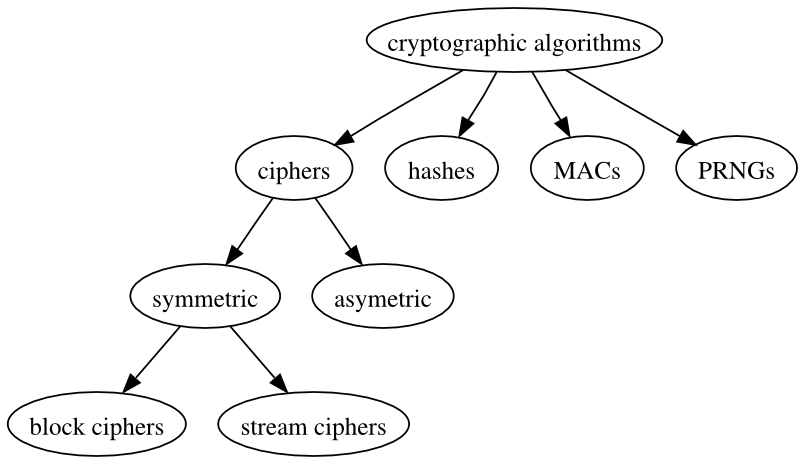
\includegraphics[width=6cm,height=5cm]{cipheroverview}
\end{frame}

\section{block ciphers}
\begin{frame}
	\frametitle{block ciphers}
	block ciphers encrypt plaintext of a fixed length (64 bit and 128 bit are quite common)
	\begin{figure}
	 \begin{minipage}[b]{.4\linewidth}
		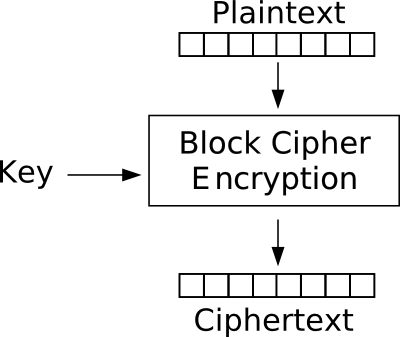
\includegraphics[width=4.5cm,height=3.5cm]{Encryption}
	 \end{minipage}
	 \hspace{.1\linewidth}
	 \begin{minipage}[b]{.4\linewidth}
		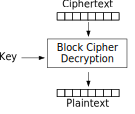
\includegraphics[width=4.5cm,height=3.5cm]{Decryption}
	 \end{minipage}
	\end{figure}
\end{frame}

\begin{frame}
\frametitle{structures of block ciphers}
	\begin{itemize}
		\item rounds
		\item feistel-network
		\item substitution-perumation-network
	\end{itemize}
\end{frame}

% ----

\begin{frame}
\frametitle{feistel-network}
	$L_{i+1} = R_i $ \\
	$R_{i+1} = L_i \oplus f(R_i, K_i)$
	\begin{center}
		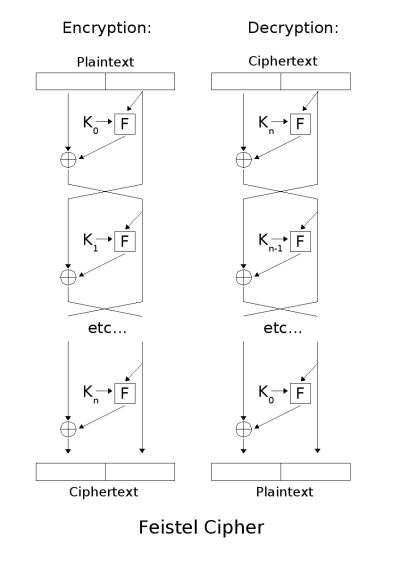
\includegraphics[scale=0.3]{Feistel}
	\end{center}
\end{frame}

%-----

\begin{frame}
\frametitle{S-Boxes}
	simple substituation function\\
	brings nonliearity\\
	mostly implemented as lookuptables
\end{frame}

%------

\begin{frame}
\frametitle{sample S-Boxe}
% \begin{tabular}{r|*{16}{r}}
%    &  0 &  1 &  2 &  3 &  4 &  5 &  6 &  7 &  8 &  9 & 10 & 11 & 12 & 13 & 14 & 15 \\ \hline
%  0 & 14 &  4 & 13 &  1 &  2 & 15 & 11 &  8 &  3 & 10 &  6 & 12 &  5 &  9 &  0 &  7 \\
%  1 &  0 & 15 &  7 &  4 & 14 &  2 & 13 &  1 & 10 &  6 & 12 & 11 &  9 &  5 &  3 &  8 \\
%  2 &  4 &  1 & 14 &  8 & 13 &  6 &  2 & 11 & 15 & 12 &  9 &  7 &  3 & 10 &  5 &  0 \\
%  3 & 15 & 12 &  8 &  2 &  4 &  9 &  1 &  7 &  5 & 11 &  3 & 14 & 10 &  0 &  6 & 13 \\
% \end{tabular}
 $S_1$ from DES:
 \begin{tabular}{c|*{16}{c}}
    &  0 &  1 &  2 &  3 &  4 &  5 &  6 &  7 &  8 &  9 &  A &  B &  C &  D &  E &  F \\ \hline
  0 &  E &  4 &  D &  1 &  2 &  E &  B &  8 &  3 &  A &  6 &  C &  5 &  9 &  0 &  7 \\
  1 &  0 &  F &  7 &  4 &  E &  2 &  D &  1 &  A &  6 &  C &  B &  9 &  5 &  3 &  8 \\
  2 &  4 &  1 &  E &  8 &  D &  6 &  2 &  B &  F &  C &  9 &  7 &  3 &  A &  5 &  0 \\
  3 &  F &  C &  8 &  2 &  4 &  9 &  1 &  7 &  5 &  B &  3 &  E &  A &  0 &  6 &  D \\
 \end{tabular}
\end{frame}
% LFSRs
% RC4

\section{stream ciphers}
\begin{frame}
\frametitle{Properties}
	\begin{itemize}
		\item<2-> Encryption ''on-stream'' - i.e. not divided into blocks
		\item<3-> Some may be used as PRNG
		\item<4-> Some require loss-free connections
	\end{itemize}
\end{frame}
\begin{frame}
\frametitle{basic modes of operation}
	\begin{itemize}
		\item<2-> Asynchronous
		\item<3-> Synchronous
	\end{itemize}
\end{frame}

\begin{frame}
\frametitle{Asynchronous mode}
	\begin{itemize}
		\item<2-> Cipher- and/or Plaintext re-used in feedback function
		\item<3-> May be used on lossy connections
		\item<4-> Self-synchronizing
	\end{itemize}
\end{frame}


\begin{frame}
\frametitle{Synchronous mode}
	\begin{itemize}
		\item<2-> No feedback function
		\item<3-> ''Entropy'' data generated idependant from plain- \& ciphertext
		\item<4-> Implies \& requires loss-free connection
	\end{itemize}
\end{frame}

\begin{frame}
\frametitle{Reallife Applications}
	\begin{itemize}
		\item<2-> Cellphones: A5 encryption (borked, don't use!)
		\item<3-> RC4 (i.e. WEP)
		\item<4-> E0 (i.e. Bluetooth)
	\end{itemize}
\end{frame}



\section{Hashfunktionen}

\begin{frame}
	\frametitle{Was sie tun}
	Eigenschaften
	\begin{columns}
	\column{6cm}
		\begin{itemize}
			\item Surjektiv \begin{small}(Eindeutige Abbildung)\end{small}
			\item Kollisionsfrei
			\item Lawineneffekt
		\end{itemize}
	\column{6cm}
		\begin{center}
			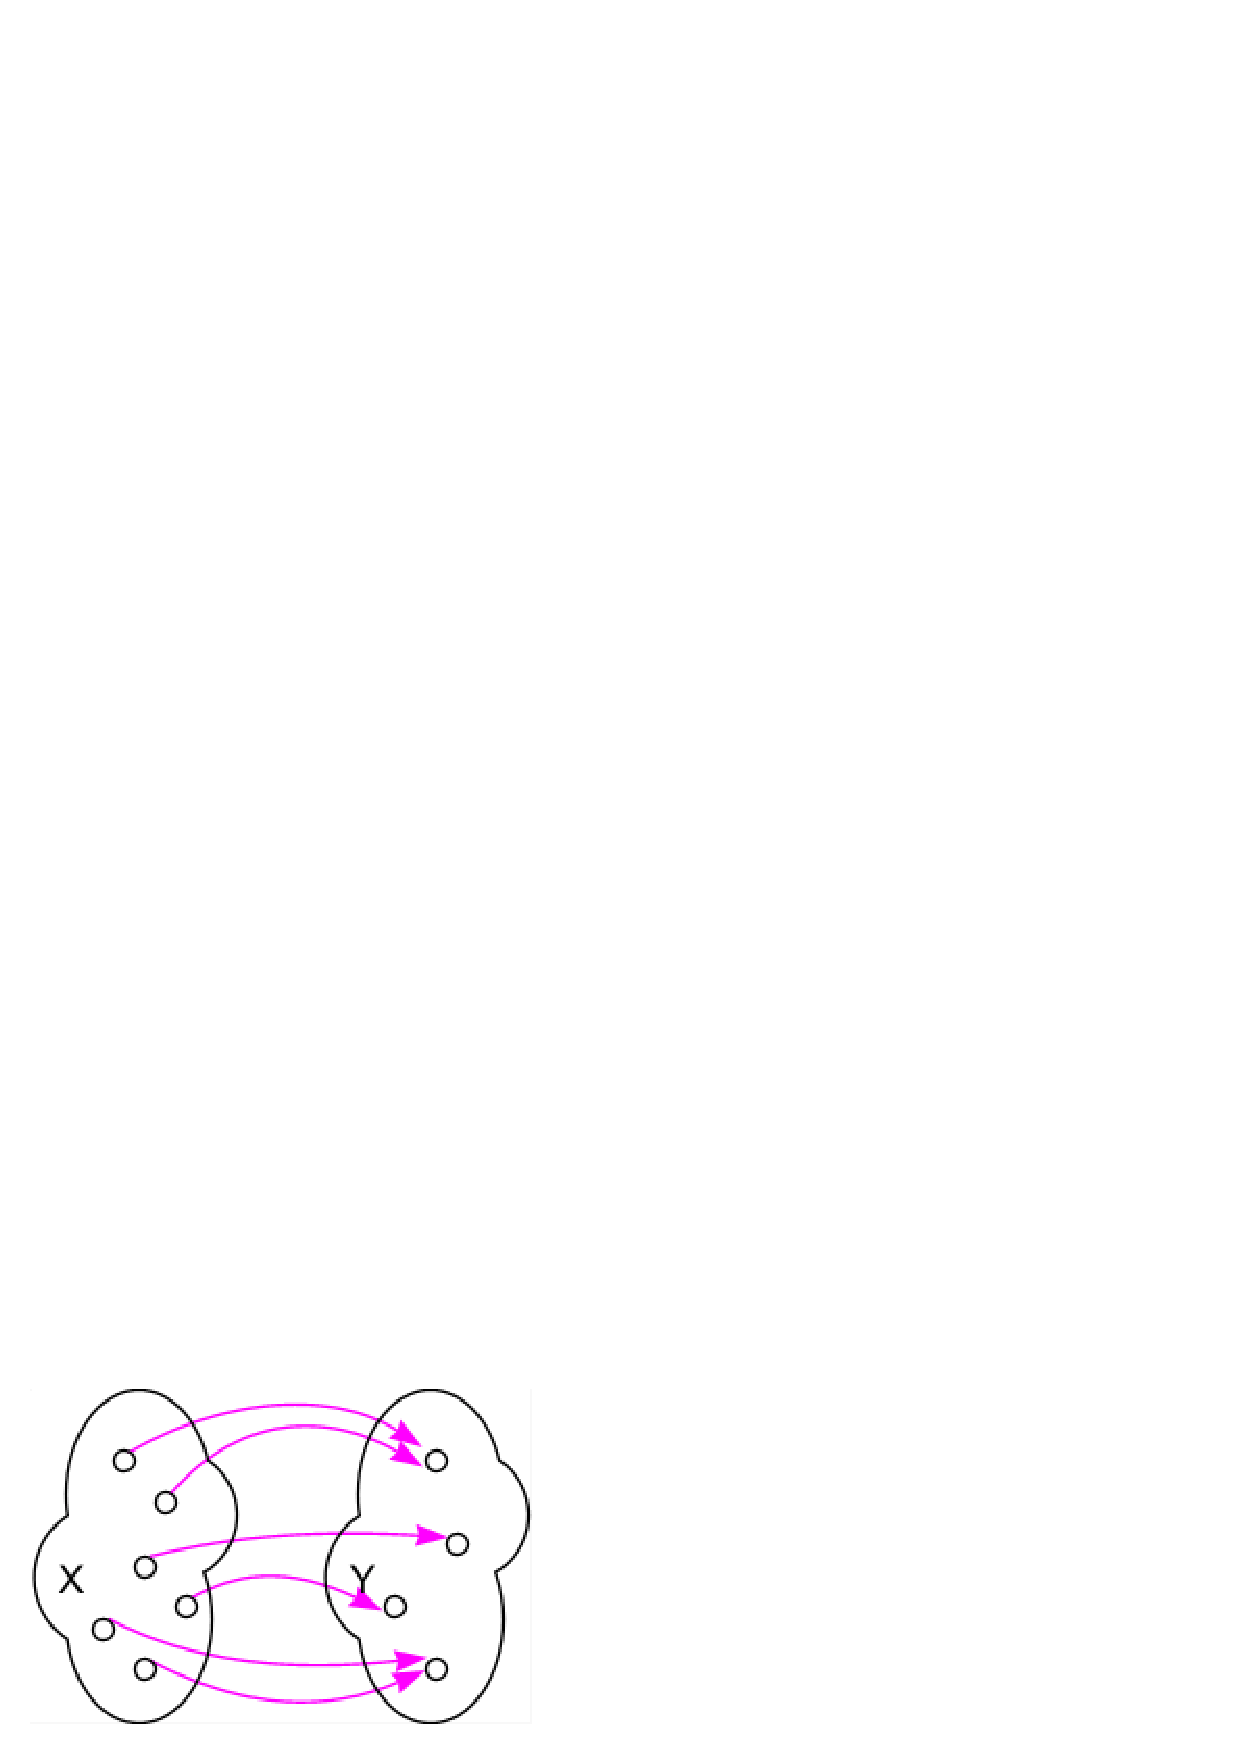
\includegraphics[width=4.8cm,height=3.2cm]{surjektiv}
		\end{center}
	\end{columns}
\end{frame}

\begin{frame}
	\frametitle{Wof"ur?}
	Was bringt's?
	\begin{itemize}
		\item Integrit"at
		\item Authenzit"at \small{(eingeschr"ankt)}
	\end{itemize}

\end{frame}

\begin{frame}
\frametitle{Warum?}
	\begin{columns}
	\column{6cm}
		\begin{itemize}
			\item One-way Eigenschaft
			\item Sinnvoll f"ur gro"se Nachrichten
		\end{itemize}
	\column{6cm}
		\begin{center}
			
\includegraphics[width=4cm,height=6cm]{oneway}
		\end{center}
	\end{columns}
\end{frame}

\begin{frame}
\frametitle{Wie?}
	Signieren mit gemeinsamen Schl"ussel
	\par
	\center{\large{\texttt{hash ( key | nachricht )}}}
\end{frame}

\end{document}

\section{MACs}

\begin{frame}
	\frametitle{WTF?}
	MAC - Massage Authentification Code\\
	Kind of ''symmetric'' signature of a message.
	
	\begin{center}$MAC_k(msg)$\end{center}
	
	Propertys:
	\begin{itemize}
		\item output of constant length
		\item collision free
		\item resistant to chosen-plaintext-attack
	\end{itemize}
\end{frame}

\begin{frame}
	\frametitle{HMAC}
	Defined in \textbf{RFC 2104}
	\par
	$HMAC_k(msg) = hash((k \oplus opad) \parallel hash((k \oplus ipad)\parallel msg) )$
\end{frame}

\begin{frame}
	\frametitle{What for?}
	Authentication of messages.
\end{frame}
\section{PRNGs}
% ----

\end{document}

